% ------------------------------------------------------------------------
% CS198 Final Paper
% Project Title: Speaker Identification Using Multi-Layer Perceptron Neural Networks
% Authors: Annliza Ni�a dL. Andrada
%          Diane Felice N. Lerma
%          Christine Pamela dG. Obedencio
%          Rochelle S. Ticlao
% Date Submitted: March 20, 2000
%
% ------------------------------------------------------------------------
\documentclass[letterpaper,12pt]{report}
\usepackage[centertags]{amsmath}
\usepackage{amsfonts}
\usepackage{amssymb}
\usepackage{amsthm}
\usepackage{newlfont}
\usepackage{epsfig}
\usepackage{UPCS198} %UP Dept. of Computer Science CS198 Style
\usepackage{UPCSINC1}
\usepackage{graphicx}
\usepackage{float}
\usepackage[active]{LTX}
\hfuzz2pt
\newlength{\defbaselineskip}
\setlength{\defbaselineskip}{\baselineskip}
\newcommand{\setlinespacing}[1]
           {\setlength{\baselineskip}{#1 \defbaselineskip}}
\newcommand{\doublespacing}{\setlength{\baselineskip}
                           {2.0 \defbaselineskip}}
\newcommand{\singlespacing}{\setlength{\baselineskip}{\defbaselineskip}}
% MATH -------------------------------------------------------------------
\newcommand{\A}{{\cal A}}
\newcommand{\h}{{\cal H}}
\newcommand{\s}{{\cal S}}
\newcommand{\W}{{\cal W}}
\newcommand{\BH}{\mathbf B(\cal H)}
\newcommand{\KH}{\cal  K(\cal H)}
\newcommand{\Real}{\mathbb R}
\newcommand{\Complex}{\mathbb C}
\newcommand{\Field}{\mathbb F}
\newcommand{\RPlus}{[0,\infty)}
\newcommand{\norm}[1]{\left\Vert#1\right\Vert}
\newcommand{\essnorm}[1]{\norm{#1}_{\text{\rm\normalshape ess}}}
\newcommand{\abs}[1]{\left\vert#1\right\vert}
\newcommand{\set}[1]{\left\{#1\right\}}
\newcommand{\seq}[1]{\left<#1\right>}
\newcommand{\eps}{\varepsilon}
\newcommand{\To}{\longrightarrow}
\newcommand{\RE}{\operatorname{Re}}
\newcommand{\IM}{\operatorname{Im}}
\newcommand{\Poly}{{\cal{P}}(E)}
\newcommand{\EssD}{{\cal{D}}}
% THEOREMS ---------------------------------------------------------------
\theoremstyle{plain}
\newtheorem{thm}{Theorem}[section]
\newtheorem{cor}[thm]{Corollary}
\newtheorem{lem}[thm]{Lemma}
\newtheorem{prop}[thm]{Proposition}
\theoremstyle{definition}
\newtheorem{defn}{Definition}[section]
\theoremstyle{remark}
\newtheorem{rem}{Remark}[section]
\numberwithin{equation}{section}
\renewcommand{\theequation}{\thesection.\arabic{equation}}
\setlength{\tclineskip}{1.05\baselineskip}

\begin{document}

%\nobib
%\draft
%\nofront

\permissionfalse


\submityear{May 2019}

% ------------------------------------------------------------------------
\title{3D Reconstruction of Underwater Terrain using Stereo Vision}


\cs198 
\author{Edmund Alwin D. de Leon
}

% ------------------------------------------------------------------------
{
\forgeterr{?0000} % Don't bother with over/under-full boxes
\beforepreface
\forgeterr{?1111} % Process All Errors from Here on
}
% ------------------------------------------------------------------------
{
\typeout{Abstract}
\prefacesection{Abstract}

This paper describes a method for 3D reconstructing underwater scenes, 
specifically the terrain and its coral reefs using stereo vision. The method
 consists of preprocessing the images, extracting the foreground of the image,
 computing the disparity map, filtering the disparity map, constructing the point cloud
  from the disparity map and then meshing the point cloud.
}
% ------------------------------------------------------------------------
{
\typeout{Acknowledgements}
\prefacesection{Acknowledgement}


Thank you Dr.Pros Naval for the guidance and support.
}
% ------------------------------------------------------------------------
\afterpreface
\def\baselinestretch{1}
\setlinespacing{1.66}
% ------------------------------------------------------------------------
{
%\typeout{Introduction}
%\include{introd}
}
% ------------------------------------------------------------------------
\setlinespacing{1.66}
% ------------------------------------------------------------------------

\chapter{Introduction}

\section{Statement of the Problem}
    The rise of autonomous underwater vehicles(AUVs) paved the way for better deep-sea exploration.
 We can now gather data about the deep waters through AUVs by attaching instruments. One of the 
 instruments that are usually attached are stereo cameras. Stereo cameras are widely used for robotic 
 control and sensing, depth perception, navigation, gesture recognition, and 3D surface visualization.

The process of acquiring of good images underwater is not simple and faces a lot of challenges such
 as light attenuation, occlutions, bubbles and a lot more. The problem is how do we filter or take into account the problems that could
  be in the acquired underwater images in order to have a better 3D reconstruction.





\section{Significance of this Study}
  The damage that has been done to our coral reefs is ever growing. A 
worldwide study in 2008 estimated that 19 percent of the existing coral reefs has already 
been lost and a projected 17 percent more over the next 10-20 years. Most of the destruction
 of the coral reefs caused by human-related activities. 

    Further study and research has to be done in order to understand and analyze
these coral reefs in preserving and growing them altogether. In this paper, we will focus in better improving 3D reconstruction of underwater scenes, specifically the underwater terrain and its corals using stereo vision.




\section{Scope of this Study}
    This study will focus on 3D reconstruction and not the image acquisition. I will be 
utilizing the dataset given by Dr. Pros Naval. The dataset contains frames/images of
corals and underwater scenes that are already rectified. 

    The camera calibration was done by Dr. Pros Naval and he provided me the needed
parameters for the methods to be used. Python language will be used for the experiments.
 Meshlab will be used for the viewing of the 3D model.

\chapter{3D Reconstruction Method}

\section{Preprocessing}
	The images used have already been stereo rectified. We use the grabcut algorithm, 
which is based on graph cuts, to extract the foreground and mask the surrounding background.

\begin{figure}[H]
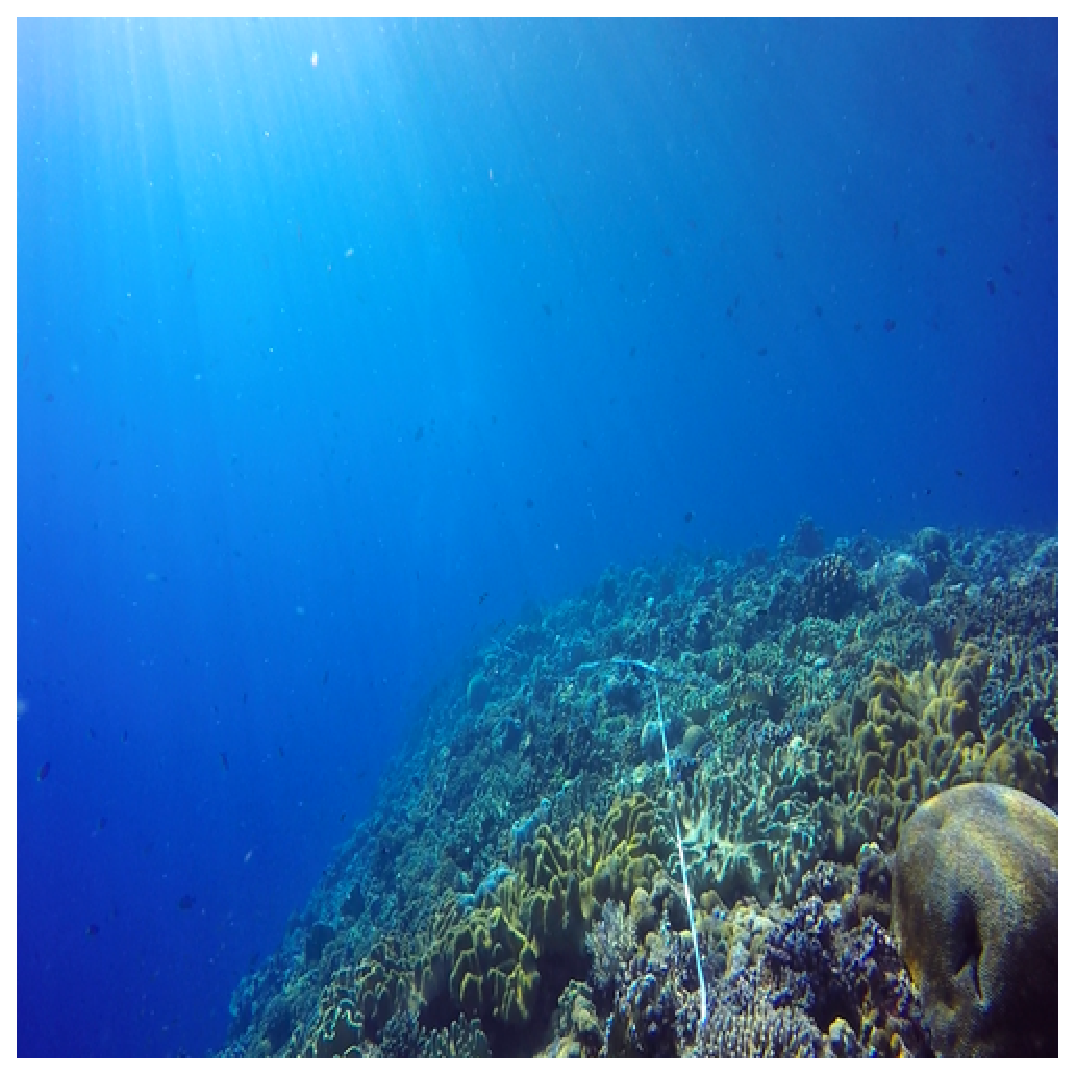
\includegraphics[width=0.8\textwidth, height=0.4\textwidth]{unmasked.eps}
\caption{Raw Rectified Image}
\end{figure}

\begin{figure}[H]

\includegraphics[width=0.8\textwidth, height=0.4\textwidth]{masked-1.eps}
\caption{Masked Rectified Image}
\end{figure}




\section{Generating the Disparity Map}

	The stereo matching algorithm used was based on Hirschmuller's, Semiglobal Matching stereo
method \cite{sgm}. It's called Semi Global Block Matching algorithm(SGBM). I tweaked the parameters for best results. After generating the disparity map, I used a weighted least squares filter to smoothen the initial dense disparity map. Next, we compute the the point cloud based from the dense disparity map.

\begin{figure}[H]

\includegraphics[width=0.8\textwidth, height=0.4\textwidth]{disp_map.eps}
\caption{Generated disparity map}
\end{figure}



\section{Interframe Reconstruction}
*not yet done*

\section{Meshing of Point Cloud}

I'm currently using Meshlab to create a mesh. The generated point cloud consists of 300,000+ points. In my meshing, I initially use poisson sampling to reduce the points and apply the ball-pivoting algorithm for surface reconstruction by Bernardini et. al.
    

\chapter{Experiments and Discussion}

The performance of the proposed method with the best selected parameters clearly shows the topography of the the terrain although the detailed
 features is not visible due to the nature of the ball-pivot algorithm. The point cloud clearly shows the features 
 and curvatures of the rocks and corals. 


\include{chapter4}
\include{chapter5}

\appendix

\chapter{Description of the Environment and Source Codes}

\section{Environment}
The program runs in the Matlab environment only. The researchers
used Matlab particularly because it contains 2 toolboxes which are
very essential to this project. These toolboxes are the Digital
Signal Processing toolbox and the Neural Network toolbox. As the
name implies, the Digital Signal Processing toolbox contains the
functions the researchers primarily used in the Speech Analysis
module -- functions like the fft, hamming, and bartlett.
Similarly, the Neural Network toolbox contains the functions used
for constructing the MultiLayer Perceptron network implemented in
this project; these functions are train, traingdx, sim, tansig,
newff, and learngdm.


\section{Interface Modules}
\subsection{Source Codes}
The following modules of the program serve as the interface of the
software.

\subsubsection{Splash}
Displays the splash screen.

\subsubsection{Main Menu}
Displays the main menu which consists of 3 choices$\:$ "Train",
"Test", and "Exit". When the user presses "Train", the program
proceeds with the module Trainparam. When the user presses "Test",
the program proceeds with another interface module, Note12. When
the user presses "Exit", the program, as well as the Matlab
environment is terminated.

\subsubsection{Trainparam}
Called upon choosing "Train" in the Main Menu. Gets the training
parameters such as the number of enrollees, number of words in the
training set, and the number of samples per word per enrollee from
the user.

\subsubsection{Get-Params}
Stores the parameters given as input in Trainparam. Stores the
parameters in 2 text files: the number of enrollees in
numEnrollees.txt and the number of words and the number of samples
per word per person in numWords.txt. Also calls the other modules
which gets the other parameters from the user such as the names of
the enrollees and words to be included in the word training set.

\subsubsection{Get-Name}
Called n times by the module Get-Params depending on the number of
enrollees. Gets the names and log-in names of the enrollees then
calls the module Store-Name to store them.

\subsubsection{Store-Name}
Also called n times depending on the number of enrollees
specified. Stores the names and log-in names given as input in
Get-Name. Stores the inputs in 2 text files: each name in
name$<$enrollee number$>$.txt and all the log-in names in
log-in.txt.

\subsubsection{Get-Word}
Called n times by the module Get-Params depending on the number of
words specified. Gets each word to be included in the word
training set then calls the module Store-Word to store the input.

\subsubsection{Store-Word}
Also called n times depending on the number of words. Stores the
words given as input in Get-Word. Creates a text file called
word-training-set.txt for the first word then simply appends the
other input words to the same text file.

\subsubsection{Note8}
Displays a note to the user of what software to use for recording
his voice, how to name the .WAV files to enable the program to use
them, where to save the .WAV files and the format by which he
should record his voice before the training. Also displays the
word training set.

\subsubsection{note12}
Called when the user chooses "Train" in the Main Menu. Same as
Note8 except it does not instruct the user on how to name the .WAV
file generated because it is not necessary to the program anymore.

\subsubsection{Decision}
Displays the decision of the testing stage. If accept, displays
the name of the speaker. If reject, displays "Sorry, but your
voice does not match any of our voice models".


\section{Speech Analysis Module}
\subsection{Source Code}
\subsubsection{Comput-Mfcc}
Called n ($n = number~of~enrollees * nnumber~of~words *
number~of~samples$) times by the Training module and called once
in the Testing module. One of the most important modules because
it reads the actual .WAV file, performs End Point Detection on the
speech signal and computes the Mel-Frequency Cepstral
Coefficients.

\subsection{Matlab Functions Used}
\subsubsection{Wavread}
function [y,Fs,bits]=wavread(file,ext)

WAVREAD Read Microsoft WAVE (".wav") sound file.

   [Y,FS,BITS]=WAVREAD(FILE) returns the sample rate (FS) in Hertz
   and the number of bits per sample (BITS) used to encode the
   data in the file.

   Supports multi-channel data, with up to 16 bits per sample.

 NOTE: This file reader only supports Microsoft PCM data format.
       It also does not support wave-list data.

\subsubsection{Hamming}
function w = hamming(n-est,sflag)

HAMMING Hamming window.

   W = HAMMING(N) returns the N-point symmetric Hamming window
       in a column vector.

\subsubsection{FFT}
FFT Discrete Fourier transform.

   FFT(X) is the discrete Fourier transform (DFT) of vector X.  If the
   length of X is a power of two, a fast radix-2 fast-Fourier
   transform algorithm is used.  If the length of X is not a
   power of two, a slower non-power-of-two algorithm is employed.
   For matrices, the FFT operation is applied to each column.
   For N-D arrays, the FFT operation operates on the first
   non-singleton dimension.

\subsubsection{Bartlett}
function w = bartlett(n-est)

BARTLETT Bartlett window.

   W = BARTLETT(N) returns the N-point Bartlett window.


\section{Classifier Modules}
\subsection{Source Codes}
The following modules implement the actual training of the neural
network and the simulation for the testing.

\subsubsection{Training}
Calls the Speech Analysis Module n times first before executing.
Concatenates all generated coefficients in one vector. Performs
the actual training of the MultiLayer Perceptron Network. Informs
the user of successful completion when finished.

\subsubsection{Testing}
Gets the .WAV input file first then calls Comput-mfcc to compute
the Mel-Frequency Cepstral Coefficients. Performs the simulation
of the MultiLayer Perceptron Network for the testing then passes
the result to the Decision module.

\subsection{Matlab Functions Used}
\subsubsection{Newff}
function net = newff(pr,s,tf,btf,blf,pf)

NEWFF Create a feed-forward backpropagation network.

   Syntax

     net = newff(PR,[S1 S2\ldots SNl],{TF1 TF2\ldots TFNl},BTF,BLF,PF)

   Description

     NEWFF(PR,[S1 S2\ldots SNl],{TF1 TF2\ldots TFNl},BTF,BLF,PF) takes,

       PR  - Rx2 matrix of min and max values for R input elements.

       Si  - Size of ith layer, for Nl layers.

       TFi - Transfer function of ith layer, default = 'tansig'.

       BTF - Backprop network training function, default = 'trainlm'.

       BLF - Backprop weight/bias learning function, default = 'learngdm'.

       PF  - Performance function, default = 'mse'.

     and returns an N layer feed-forward backprop network.

     The transfer functions TFi can be any differentiable transfer
     function such as TANSIG, LOGSIG, or PURELIN.

     The training function BTF can be any of the backprop training
     functions such as TRAINLM, TRAINBFG, TRAINRP, TRAINGD, etc.

     The learning function BLF can be either of the backpropagation
     learning functions such as LEARNGD, or LEARNGDM.

     The performance function can be any of the differentiable performance
     functions such as MSE or MSEREG.

   Algorithm

     Feed-forward networks consist of Nl layers using the DOTPROD
     weight function, NETSUM net input function, and the specified
     transfer functions.

     The first layer has weights coming from the input.  Each subsequent
     layer has a weight coming from the previous layer.  All layers
     have biases.  The last layer is the network output.

     Each layer's weights and biases are initialized with INITNW.

     Adaption is done with ADAPTWB which updates weights with the
     specified learning function. Training is done with the specified
     training function. Performance is measured according to the specified
     performance function.

\subsubsection{Tansig}
function a = tansig(n,b)

TANSIG Hyperbolic tangent sigmoid transfer function.

   Syntax

     A = tansig(N)

     info = tansig(code)

   Description

     TANSIG is a transfer function.  Transfer functions
     calculate a layer's output from its net input.

   Algorithm

     TANSIG(N) calculates its output according to:

       n = 2/(1+exp(-2*n))-1

     This is mathematically equivalent to TANH(N).  It differs
     in that it runs faster than the MATLAB implementation of TANH,
     but the results can have very small numerical differences.  This
     function is a good trade off for neural networks, where speed is
     important and the exact shape of the transfer function is not.

\subsubsection{Traingdx}
function [net,tr] = traingdx(net,Pd,Tl,Ai,Q,TS,VV,TV)

TRAINGDX Gradient descent w/momentum and adaptive lr
backpropagation.

   Syntax

     [net,tr] = traingdx(net,Pd,Tl,Ai,Q,TS,VV)
     info = traingdx(code)

   Description

     TRAINGDX is a network training function that updates weight and
     bias values according to gradient descent momentum and an
     adaptive learning rate.

     Training occurs according to the TRAINGDX's training parameters
     shown here with their default values:
       net.trainParam.epochs         10  Maximum number of epochs to train

       net.trainParam.goal            0  Performance goal

       net.trainParam.lr           0.01  Learning rate

       net.trainParam.lr-inc       1.05  Ratio to increase learning rate

       net.trainParam.lr-dec        0.7  Ratio to decrease learning rate

       net.trainParam.max-fail        5  Maximum validation failures

       net.trainParam.max-perf-inc 1.04  Maximum performance increase

       net.trainParam.mc            0.9  Momentum constant.

       net.trainParam.min-grad    1e-10  Minimum performance gradient

       net.trainParam.show           25  Epochs between showing progress

       net.trainParam.time          inf  Maximum time to train in seconds

     Dimensions for these variables are:

       Pd - NoxNixTS cell array, each element P{i,j,ts} is a DijxQ matrix.

       Tl - NlxTS cell array, each element P{i,ts} is an VixQ matrix.

       Ai - NlxLD cell array, each element Ai{i,k} is an SixQ matrix.

     Where

       Ni = net.numInputs

       Nl = net.numLayers

       LD = net.numLayerDelays

       Ri = net.inputs{i}.size

       Si = net.layers{i}.size

       Vi = net.targets{i}.size

       Dij = Ri * length(net.inputWeights{i,j}.delays)

     If VV is not [], it must be a structure of validation vectors,

       VV.PD - Validation delayed inputs.

       VV.Tl - Validation layer targets.

       VV.Ai - Validation initial input conditions.

       VV.Q  - Validation batch size.

       VV.TS - Validation time steps.

     which is used to stop training early if the network performance
     on the validation vectors fails to improve or remains the same
     for MAX-FAIL epochs in a row.

   Algorithm

     TRAINGDX can train any network as long as its weight, net input,
     and transfer functions have derivative functions.

     Backpropagation is used to calculate derivatives of performance
     PERF with respect to the weight and bias variables X.  Each
     variable is adjusted according to the gradient descent
     with momentum.

       dX = mc*dXprev + lr*mc*dperf/dX

     where dXprev is the previous change to the weight or bias.

     For each epoch, if performance decreases toward the goal, then
     the learning rate is increased by the factor lr-inc.  If
    performance increases by more than the factor max-perf-inc,
     the learning rate is adjusted by the factor lr-dec and the
     change, which increased the performance, is not made.

     Training stops when any of these conditions occur:

     1) The maximum number of EPOCHS (repetitions) is reached.

     2) The maximum amount of TIME has been exceeded.

     3) Performance has been minimized to the GOAL.

     4) The performance gradient falls below MINGRAD.

     5) Validation performance has increase more than MAX-FAIL times
        since the last time it decreased (when using validation).

\subsubsection{Train}
function [net,tr]=train(net,P,T,Pi,Ai,VV,TV)

TRAIN Train a neural network.

   Syntax

     [net,tr] = train(NET,P,T,Pi,Ai)

     [net,tr] = train(NET,P,T,Pi,Ai,VV,TV)

   Description

     TRAIN trains a network NET according to NET.trainFcn and
     NET.trainParam.

     TRAIN(NET,P,T,Pi,Ai) takes,

       NET - Network.

       P   - Network inputs.

       T   - Network targets, default = zeros.

       Pi  - Initial input delay conditions, default = zeros.

       Ai  - Initial layer delay conditions, default = zeros.

     and returns,

       NET - New network.

       TR  - Training record (epoch and perf).

     TRAIN(NET,P,T,Pi,Ai,VV,TV) takes optional structures of validation
     and test vectors,

       VV.P,  TV.P  - Validation/test inputs.

       VV.T,  VV.T  - Validation/test targets, default = zeros.

       VV.Pi, VV.Pi - Validation/test initial input delay conditions, default = zeros.

       VV.Ai, VV.Ai - Validation/test layer delay conditions, default = zeros.

     The validation vectors are used to stop training early if further
     training on the primary vectors will hurt generalization to the
     validation vectors.  Test vector performance can be used to measure
     how well the network generalizes beyond primary and validation vectors.
     If VV.T, VV.Pi, or VV.Ai are set to an empty matrix or cell array,
     default values will be used. The same is true for VT.T, VT.Pi, VT.Ai.

   Algorithm

     TRAIN calls the function indicated by NET.trainFcn, using the
     adaption parameter values indicated by NET.trainParam.

     Typically one epoch of training is defined as a single presentation
     of all input vectors to the network.  The network is then updated
     according to the results of all those presentations.

     Training occurs until a maximum number of epochs occurs, the
     performance goal is met, or any other stopping condition of the
     function NET.trainFcn occurs.

     Some training functions depart from this norm by presenting only
     one input vector (or sequence) each epoch. An input vector (or sequence)
     is chosen randomly each epoch from concurrent input vectors (or sequences).
     NEWC and NEWSOM return networks that use TRAINWB1, a training function
     that does this.

\subsubsection{Sim}
function [Y,Pf,Af]=sim(net,P,Pi,Ai)

SIM Simulate a neural network.

   Syntax

     [Y,Pf,Af] = sim(net,P,Pi,Ai)

     [Y,Pf,Af] = sim(net,{Q TS},Pi,Ai)

     [Y,Pf,Af] = sim(net,Q,Pi,Ai)

   Description

     SIM simulates neural networks.

     [Y,Pf,Af] = SIM(net,P,Pi,Ai) takes,

       NET - Network.

       P   - Network inputs.

       Pi  - Initial input delay conditions, default = zeros.

       Ai  - Initial layer delay conditions, default = zeros.

     and returns:

       Y   - Network outputs.

       Pf  - Final input delay conditions.

       Af  - Final layer delay conditions.

     [Y,Pf,Af] = SIM(net,{Q TS},Pi,Ai)

     is used for networks which do not have an input, such
     as Hopfield networks when cell array notation is used.

     [Y,Pf,Af] = SIM(net,Q,Pi,Ai) is used for networks
     which do not have an input, such as Hopfield networks
     when matrix notation is used.

   Algorithm

     SIM uses these properties to simulate a network NET.

       NET.numInputs, NET.numLayers

       NET.outputConnect, NET.biasConnect

       NET.inputConnect, NET.layerConnect

     These properties determine the network's weight and bias values,
     and the number of delays associated with each weight:

       NET.inputWeights{i,j}.value

       NET.layerWeights{i,j}.value

       NET.layers{i}.value

       NET.inputWeights{i,j}.delays

       NET.layerWeights{i,j}.delays

     These function properties indicate how SIM applies weight and
     bias values to inputs to get each layer's output:

       NET.inputWeights{i,j}.weightFcn

       NET.layerWeights{i,j}.weightFcn

       NET.layers{i}.netInputFcn

       NET.layers{i}.transferFcn

\subsubsection{Learngdm}
function [dw,ls] = learngdm(w,p,z,n,a,t,e,gW,gA,d,lp,ls)

LEARNGDM Gradient descent w/momentum weight/bias learning
function.

   Syntax

     [dW,LS] = learngdm(W,P,Z,N,A,T,E,gW,gA,D,LP,LS)

     [db,LS] = learngdm(b,ones(1,Q),Z,N,A,T,E,gW,gA,D,LP,LS)

     info = learngdm(code)

   Description

     LEARNGDM is the gradient descent with momentum weight/bias
     learning function.

     LEARNGDM(W,P,Z,N,A,T,E,gW,gA,D,LP,LS)

     takes several inputs,

       W  - SxR weight matrix (or Sx1 bias vector).

       P  - RxQ input vectors (or ones(1,Q)).

       Z  - SxQ weighted input vectors.

       N  - SxQ net input vectors.

       A  - SxQ output vectors.

       T  - SxQ layer target vectors.

       E  - SxQ layer error vectors.

       gW - SxR gradient with respect to performance.

       gA - SxQ output gradient with respect to performance.

       D  - SxS neuron distances.

       LP - Learning parameters, none, LP = [].

       LS - Learning state, initially should be = [].

     and returns,

       dW - SxR weight (or bias) change matrix.

       LS - New learning state.

     Learning occurs according to LEARNGDM's learning parameters,
     shown here with their default values.

       LP.lr - 0.01 - Learning rate

       LP.mc - 0.9  - Momentum constant

     LEARNGDM(CODE) returns useful information for each CODE string:

       'pnames'    - Returns names of learning parameters.

       'pdefaults' - Returns default learning parameters.

       'needg'     - Returns 1 if this function uses gW or gA.

   Algorithm

     LEARNGDM calculates the weight change dW for a given neuron
     from the neuron's input P and error E, the weight (or bias)
     learning rate LR, and momentum constant MC, according to
     gradient descent with momentum:

       dW = mc*dWprev + (1-mc)*lr*gW

     The previous weight change dWprev is stored and read
     from the learning state LS.


% ------------------------------------------------------------------------
%\INPUT{thesis.bib}

\setlinespacing{1.44}
\bibliographystyle{plain}
\bibliography{biblio}


\end{document}
